\documentclass[12pt,letterpaper]{article}

\usepackage{graphicx}
\usepackage[utf8]{inputenc}
\usepackage{mathtools}
\usepackage[margin=0.5in]{geometry}
\usepackage{booktabs}
\usepackage{tabu}
\usepackage{caption}
\usepackage[labelfont=bf, skip=5pt, font=small]{caption}
\usepackage{hyperref}
\usepackage{siunitx}
\usepackage{standalone}
\usepackage{import}
\usepackage{stanli}


\hypersetup{
    colorlinks=true,
    linkcolor=blue,
    filecolor=magenta,      
    urlcolor=cyan,
    pdftitle={Overleaf Example},
    pdfpagemode=FullScreen,
    }
\usepackage[font=footnotesize,labelfont=bf]{caption}
\setlength{\parskip}{1em}
\setlength{\parindent}{0em}




\let\DeclareUSUnit\DeclareSIUnit
\let\US\SI
\DeclareUSUnit\inch{in}
\DeclareUSUnit\lbf{lbf}
\DeclareUSUnit\lb{lb}
\DeclareUSUnit\psi{psi}
\DeclareUSUnit\ksi{ksi}
\DeclareUSUnit\Msi{Msi}











\begin{document}
\subsubsection{Landing Gear}

There are a couple different types of landing gear typically used on landers, shown bellow.

\begin{figure}[h!]
\centering
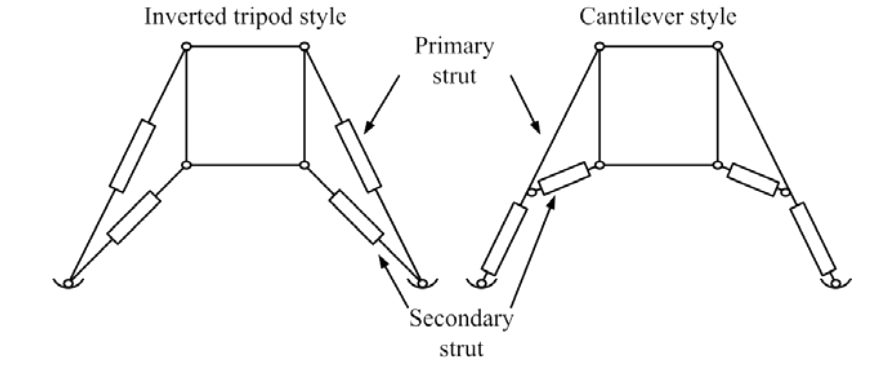
\includegraphics[width = 0.75\textwidth]{Landing_Legs_Fig/types_of_landing_legs.png}
\end{figure}

Based on research (\href{https://books.google.com/books?id=Pe4lEAAAQBAJ&pg=PA379&lpg=PA379&dq=cantilever+vs+tripod+landing+gear+lander&source=bl&ots=DuGdF26dV6&sig=ACfU3U2t155w4LoJxWtv7OWv5jt4EfvQcA&hl=en&sa=X&ved=2ahUKEwib4qHcyIv6AhWbKkQIHW6DAAwQ6AF6BAggEAM#v=onepage&q=cantilever%20vs%20tripod%20landing%20gear%20lander&f=false}{Paper 1} , \href{https://ltu.diva-portal.org/smash/get/diva2:1159285/FULLTEXT01.pdf}{Paper 2}) the tripod design offers the best specific strength  and simpler analysis for small landers. This makes logical sense, as it is essentially just a truss. For this design no damping will be used.

The first question that needs answering to eventually get to the exact geometry of the landing gear, is how big does my landing radius need to be? The landing radius as I am defining it, is based on the circle that intersects each foot of the landing gear. The minimum effective tip-over radius is defined by the number of legs in this given landing radius. The more legs that are added, the closer the minimum effective tip-over radius comes to the landing radius. This is important in calculating your worst case tip over. The worst case tip over will exist about the axis defined by a line between any two neighboring legs around the landing radius. 

\begin{figure}[h!]
\centering
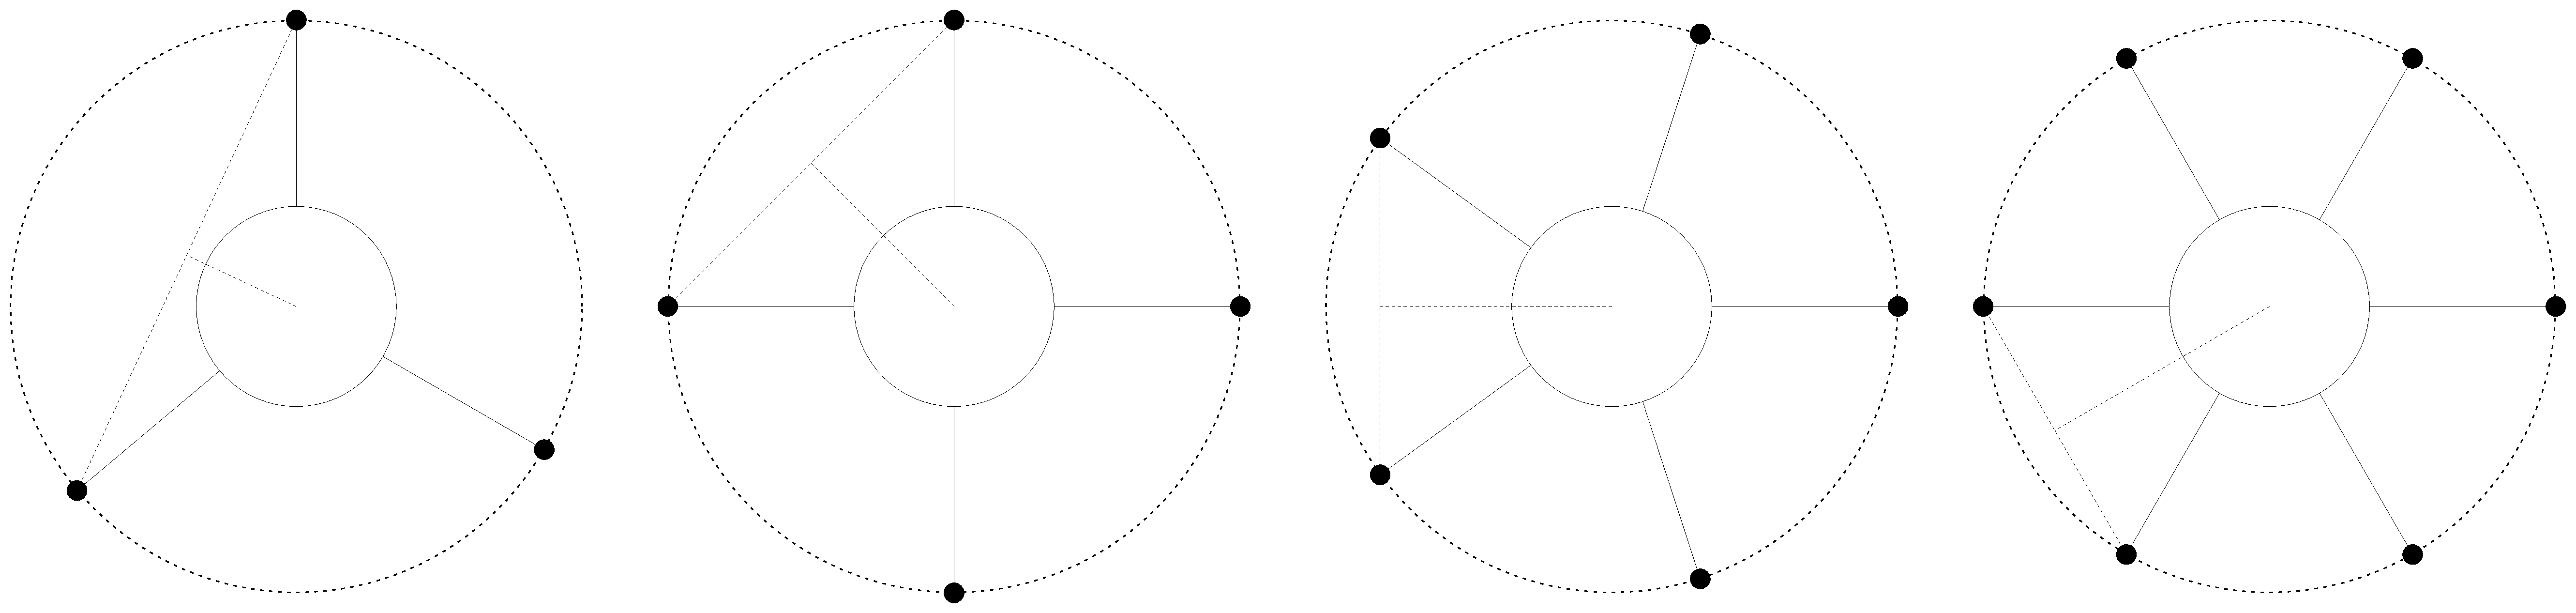
\includegraphics[width = 0.75\textwidth]{Landing_Legs_Fig/Landing_Radius.pdf}
\end{figure}

Four legs was chosen for this vehicle, due to motor mounts geometric constraints. This allows the landing legs to stay integrated, symmetric and a consistent with the rest of the vehicle frame.

Because landing is a complicated dynamic problem, I will be simplifying by choosing a large static tip over angle in the hopes that this results in a large enough effective landing radius, to compensate for the complex behavior. In order to design more carefully, I would need to estimate potential side forces, kinetic friction of the landing surface and run rigid body simulations to accurately access dynamic tip over. Instead , I have chosen a static tip over angle of 50\unit{\degree} from horizontal. Because my landing gear is both symmetrical and square, I can also represent this in 2D without projecting a effective landing radius (this is not the case for different amounts of legs). This means that the minimum effective landing width ($l_w$), must not exceed the value calculated value in Equation(1).

\pagebreak

\begin{figure}[h!]
\centering
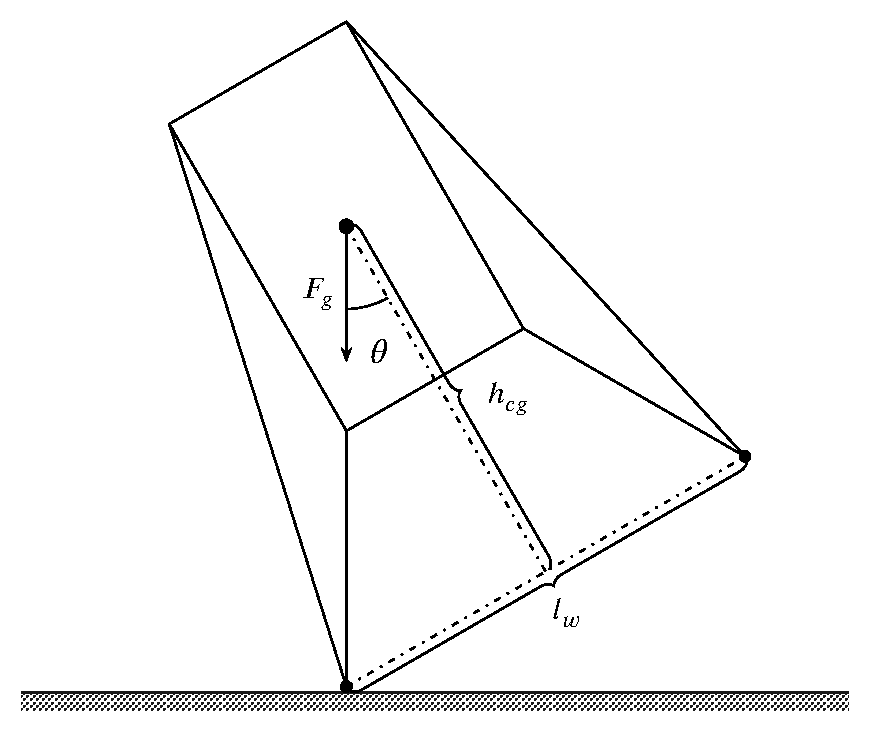
\includegraphics[width = 0.45\textwidth]{Landing_Legs_Fig/Tip_Over.pdf}
\end{figure}
\begin{description}
    \item $\theta = $ Tip Over Angle 
    \item $h_{cg} =$ Height of the Center of Gravity 
    \item $l_w = $ Effective Landing Width
    \item $F_g$ = Force of Gravity
\end{description}

\begin{equation}
    l_w = 2 h_{cg} \sin{\theta}
\end{equation}

The height of the center of gravity with respect to the landing gear, is equal to the current height of the structure of the vehicle, plus a chosen two and a half inches of ground clearance. After the major mass components had finished design, this height came out to 8.947\unit{\inch}.

\begin{gather*}
    \centering
    l_w = 2 * 8.947\unit{\inch} * \sin{50^\circ}
\end{gather*}
\begin{gather*}
    \centering
    l_w = 13.7\unit{\inch}
\end{gather*}

From this, using the derived sketch of the vehicle, the ground clearance and effective landing radius can be defined to generate the base coordinates of the landing gear truss members.

Estimated landing forces, as I have found is extremely difficult without building something, simulating something or using expensive analysis software. Originally, I was going to use a hand calculation based on the assumption of a inelastic collision with the ground. Unfortunately, this requires a major assumption about the time duration of the impact. Resources online vary wildly for how long an impact takes to decelerate a body, a difference of a couple milliseconds can vary the load by a factor of more than 100. I attempted to measure impact accelerations and estimate this time, using a drone dropped from various heights however the mems accelerometer that I am using even at its max full scale range of +-16gs, provided saturated and untrustworthy data of around 4gs. For this reason I will be adding a conservative fudge factor of 2 onto that measure figure (8gs). This is not accurate is simply a judgment call, for the purposes of future vehicle designs. I will be building a dedicated test stand to measure impact loads on landing. I will adjust the landing leg design once I have a better idea what these loads are. 


\pagebreak

\begin{figure}[h!]
\centering
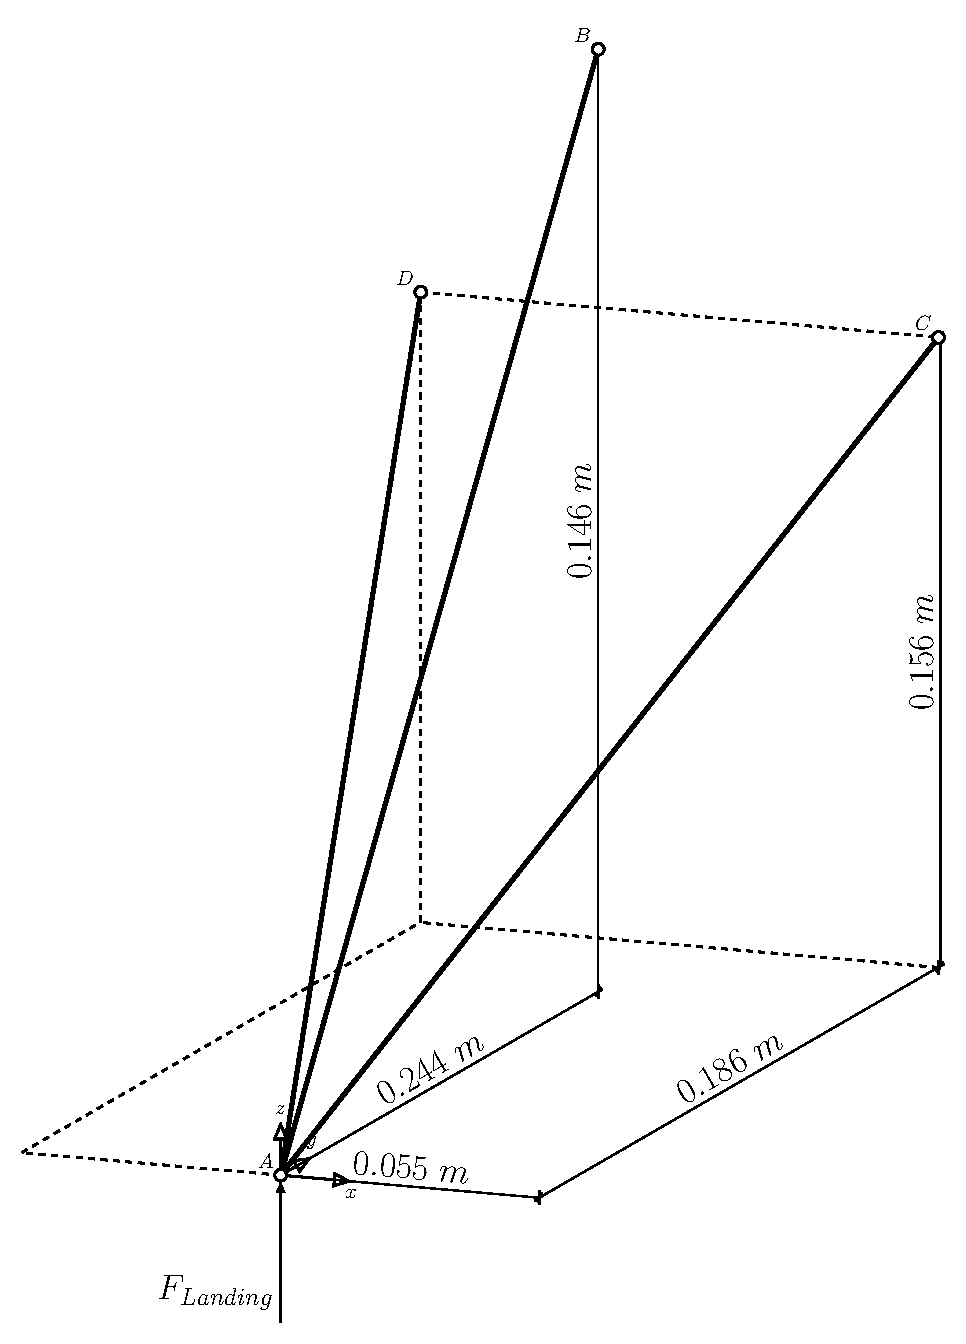
\includegraphics[width = 0.45\textwidth]{Landing_Legs_Fig/Landing_Leg_Truss.pdf}
\caption{Landing Leg Truss}
\end{figure}


Using the current estimated mass of the vehicle without landing legs (an assumption that needs to be considered for the FOS later, landing gear may increase the vehicle mass by 10\%) of 591.58\unit{\g}, the following landing load on the vehicle was calculated:

\begin{gather*}
    F_l~=~8g~m_v~=~8~*~9.8055\unit[per-mode = fraction]{\m\per\s\squared} * 0.59158\unit{\kg} = 46.4\unit{\N}
\end{gather*}

Now that the landing load is known, the problem is statically determinate and requires only analysis at the foot joint.

\pagebreak

\begin{figure}[h!]
\centering
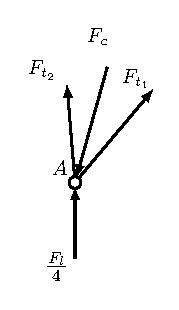
\includegraphics[width = 0.15\textwidth]{Landing_Legs_Fig/FBD_point_A.pdf}
\end{figure}


\begin{description}
    \item Vector Components:
    \item $\frac{F_l}{4}$ [0i + 0j + 1k]
    \item $F_c$ [0i + 0.51282263j  + 0.85849458k]
    \item $F_{t_1}$ [0.22127908i + 0.74661525j + 0.62737647k]
    \item $F_{t_2}$ = $F_2$ [-0.2212790i + 0.74661525j + 0.62737647k]
\end{description}

Assuming all members are in tension (despite the intuition shown in the FBD) the following static equations can be derived:

\begin{gather}
\begin{aligned}
    & \Sigma F_i~=~F_{t_1}i~-~F_{t_1}i~=~0
    \\
    & \Sigma F_j~=~F_cj~+~2~F_{t_1}j~=~0 
    \\
    & \Sigma F_k~=~\frac{F_l}{4}k~+~F_ck~+~2F_{t_1}k~=~0 
\end{aligned}
\end{gather}

Supplementing the design figure of landing force and simplifying:
\begin{gather*}
\begin{aligned}
   & \frac{F_l}{4}k~=~11.6\unit{\N}
    \\
    & 0.512~F_c~+~1.493~F_{t_1}~=~0 
    \\
    & 0.858~F_c~+~1.254~F_{t_1}~= -11.6\unit{\N}
\end{aligned}
\end{gather*}
Solving the system of equations:

\begin{gather*}
\begin{aligned}
	& F_c = -27.15\unit{\N}
	\\
    &F_{t_1} = F_{t_2} = 9.32\unit{\N}
\end{aligned}
\end{gather*}

Negative values indicate the member is in compression. Its important to note at this point that the actual assembly is not the ideal truss, there are slight eccentric loads and the members will not be in perfect axial loading conditions as assumed in this model. For this reason I will be using higher FOS than usual. Additionally, the initial results of this optimization showed cross sections that where very small in the tension. This small cross section made me concerned about deflection, this has been added to the optimization. Deflection was not a consideration for the compression members.  

Now that the loads have been established, an optimization for the minimum weight member given a circular cross section can be preformed based on the following design factors.
\\
\begin{description}
	\item Compression Member:
	\begin{description}
		\item Failure Mode = Buckling	
    		\item Target Factor of Safety on Ultimate = 4
	\end{description}
  	\item Tension Members:
  	\begin{description}
  		\item Failure Mode = Tensile
    		\item Target Factor of Safety on Ultimate = 2.5
    		\item Target Displacement = 0.0025\unit{\m}
  	\end{description}
\end{description}

\begin{figure}[h!]
\centering
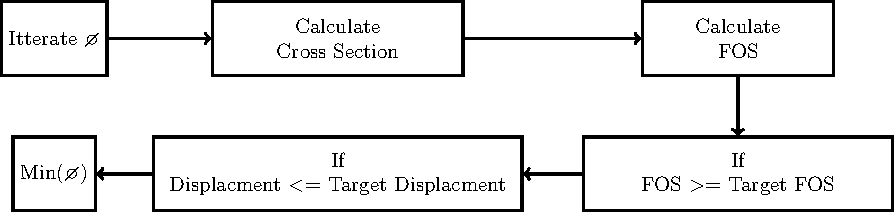
\includegraphics[width = 0.75\textwidth]{Landing_Legs_Fig/Landing_Leg_Optimization_Logic.pdf}
\end{figure}


The material trade was not in depth for this part, carbon fiber seemed to be the logical choice for both integration and mass.

Results:

\begin{description}
\item Compression Member:
    \begin{description}
        \item Diameter =  0.003358\unit{\m}
        \item Factor of Safety = 4
    \end{description}
\item Tension Members:
    \begin{description}
        \item Diameter = 0.00029\unit{\m}
        \item Factor of Safety = 11.3
        \item Displacement = 0.0025\unit{\m} 
    \end{description}
\end{description}

Based on the available carbon rods the final size choice is:

%https://www.cstsales.com/carbon_rods.html
\begin{description}
	\item Compression Member Diameter = 3.45\unit{\mm} (0.136\unit{\inch})
	\item Tension Member's Diameter = 0.5\unit{\mm} (0.020\unit{\inch})
\end{description}

\pagebreak

\begin{figure}[h!]
\centering
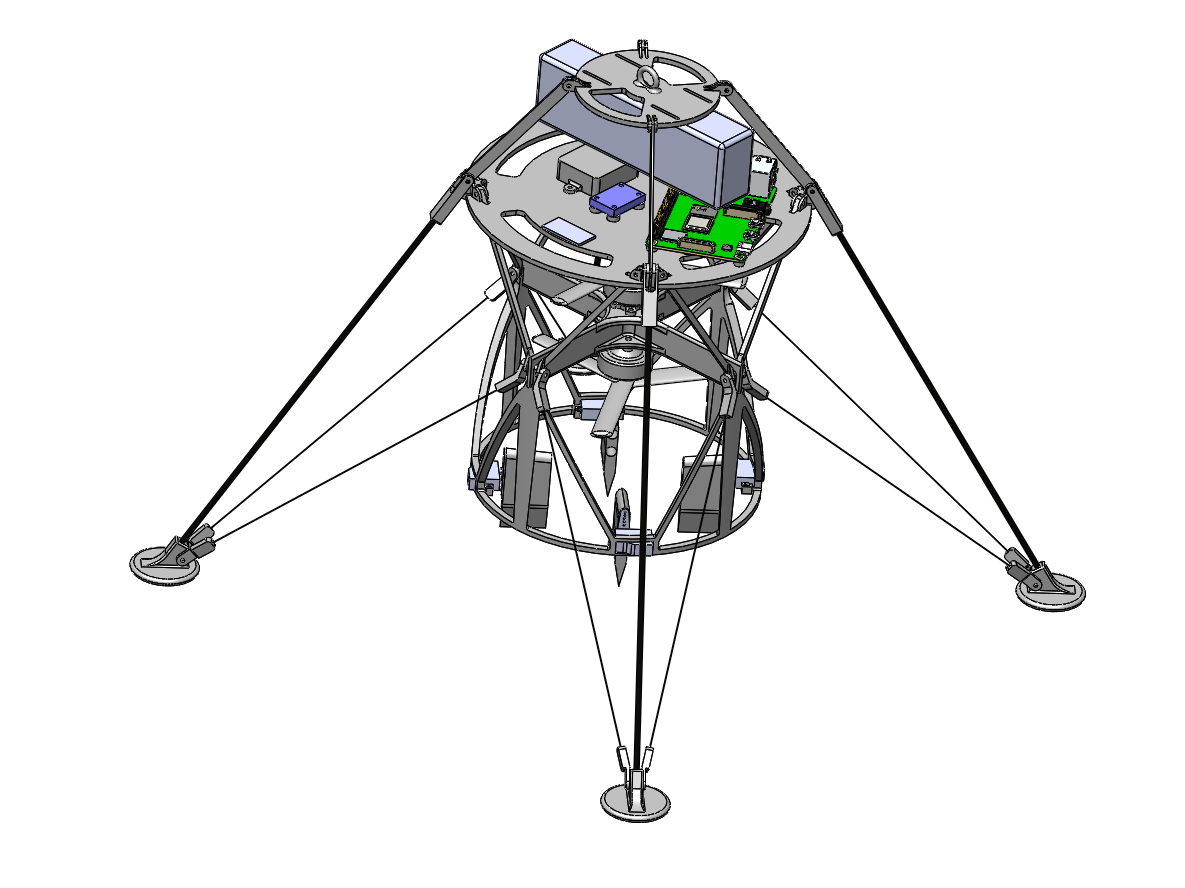
\includegraphics[width = 0.9\textwidth]{Landing_Legs_Fig/End.png}
\caption*{Design as of 09/10/22}
\end{figure}







\end{document}
